\chapter{Conception} \label{Chapter3}

\section{Dictionnaire de données}

\begin{table}[ht!]
\centering
\resizebox{\columnwidth}{!}{%
\begin{tabular}{c|lllcl|}
\cline{2-6}
\multicolumn{1}{l|}{} &
  \multicolumn{5}{c|}{{\color[HTML]{000000} \textbf{Dictionnaire de données}}} \\ \cline{2-6}
\multicolumn{1}{l|}{} &
  \multicolumn{1}{c|}{\textbf{Nom symbolique}} &
  \multicolumn{1}{c|}{\textbf{Signification}} &
  \multicolumn{1}{c|}{\textbf{Type}} &
  \multicolumn{1}{c|}{\textbf{Taille}} &
  \multicolumn{1}{c|}{\textbf{Contraintes, règles de calcul}} \\ \hline
\multicolumn{1}{|c|}{} &
  \multicolumn{1}{l|}{{\ul \textbf{user\_id}}} &
  \multicolumn{1}{l|}{ID d'utilisateur} &
  \multicolumn{1}{l|}{Numérique} &
  \multicolumn{1}{c|}{100} &
  Automatique \\
\multicolumn{1}{|c|}{} &
  \multicolumn{1}{l|}{user\_nom} &
  \multicolumn{1}{l|}{Nom de l'utilisateur} &
  \multicolumn{1}{l|}{Alphanumérique} &
  \multicolumn{1}{c|}{50} &
  Obligatoire \\
\multicolumn{1}{|c|}{} &
  \multicolumn{1}{l|}{user\_email} &
  \multicolumn{1}{l|}{Adresse mail utilisateur} &
  \multicolumn{1}{l|}{Alphanumérique} &
  \multicolumn{1}{c|}{50} &
   \\
\multicolumn{1}{|c|}{} &
  \multicolumn{1}{l|}{user\_password} &
  \multicolumn{1}{l|}{Mot de passe utilisateur} &
  \multicolumn{1}{l|}{Alphanumérique} &
  \multicolumn{1}{c|}{50} &
  Obligatoire \\
\multicolumn{1}{|c|}{\multirow{}{}{\textbf{Utilisateur}}} &
  \multicolumn{1}{l|}{user\_derniere\_session} &
  \multicolumn{1}{l|}{Dernière sessios} &
  \multicolumn{1}{l|}{Date} &
  \multicolumn{1}{c|}{8} &
  Forme JJ-MM-AAAA \\ \hline
\multicolumn{1}{|c|}{} &
  \multicolumn{1}{l|}{{\ul \textbf{produit\_id}}} &
  \multicolumn{1}{l|}{ID produit} &
  \multicolumn{1}{l|}{Numérique} &
  \multicolumn{1}{c|}{100} &
  Automatique \\
\multicolumn{1}{|c|}{} &
  \multicolumn{1}{l|}{libelle\_produit} &
  \multicolumn{1}{l|}{Libellé produit} &
  \multicolumn{1}{l|}{Alphanumérique} &
  \multicolumn{1}{c|}{50} &
  Obligatoire \\
\multicolumn{1}{|c|}{} &
  \multicolumn{1}{l|}{produit\_temperature\_max} &
  \multicolumn{1}{l|}{Température maximal} &
  \multicolumn{1}{l|}{Numérique} &
  \multicolumn{1}{c|}{100} &
  Obligatoire, \textgreater 0 \\
\multicolumn{1}{|c|}{} &
  \multicolumn{1}{l|}{produit\_temperature\_min} &
  \multicolumn{1}{l|}{Température minimal} &
  \multicolumn{1}{l|}{Numérique} &
  \multicolumn{1}{c|}{100} &
  Obligatoire, \textgreater 0 \\
\multicolumn{1}{|c|}{\multirow{}{}{\textbf{Produit}}} &
  \multicolumn{1}{l|}{produit\_description} &
  \multicolumn{1}{l|}{Description du produit} &
  \multicolumn{1}{l|}{Alphanumérique} &
  \multicolumn{1}{c|}{100} &
  Obligatoire \\ \hline
\multicolumn{1}{|c|}{} &
  \multicolumn{1}{l|}{{\ul \textbf{catégorie\_id}}} &
  \multicolumn{1}{l|}{ID du catégorie} &
  \multicolumn{1}{l|}{Numérique} &
  \multicolumn{1}{c|}{100} &
  Automatique \\
\multicolumn{1}{|c|}{\multirow{}{}{\textbf{Catégorie}}} &
  \multicolumn{1}{l|}{libelle\_catégorie} &
  \multicolumn{1}{l|}{Libellé catégorie} &
  \multicolumn{1}{l|}{Alphanumérique} &
  \multicolumn{1}{c|}{50} &
  Obligatoire \\ \hline
\multicolumn{1}{|c|}{} &
  \multicolumn{1}{l|}{{\ul \textbf{taille\_id}}} &
  \multicolumn{1}{l|}{ID taille} &
  \multicolumn{1}{l|}{Numérique} &
  \multicolumn{1}{c|}{100} &
  Automatique \\
\multicolumn{1}{|c|}{} &
  \multicolumn{1}{l|}{libelle\_taille} &
  \multicolumn{1}{l|}{Libellé de la taille} &
  \multicolumn{1}{l|}{Numérique} &
  \multicolumn{1}{c|}{100} &
  Obligatoire, \textgreater 0 \\
\multicolumn{1}{|c|}{} &
  \multicolumn{1}{l|}{taille\_hauteur} &
  \multicolumn{1}{l|}{Hauteur du produit} &
  \multicolumn{1}{l|}{Numérique} &
  \multicolumn{1}{c|}{100} &
  Obligatoire, \textgreater 0 \\
\multicolumn{1}{|c|}{} &
  \multicolumn{1}{l|}{taille\_largeur} &
  \multicolumn{1}{l|}{Largeur du produit} &
  \multicolumn{1}{l|}{Numérique} &
  \multicolumn{1}{c|}{100} &
  Obligatoire, \textgreater 0 \\
\multicolumn{1}{|c|}{\multirow{}{}{\textbf{Taille}}} &
  \multicolumn{1}{l|}{volume} &
  \multicolumn{1}{l|}{Volume du produit} &
  \multicolumn{1}{l|}{Numérique} &
  \multicolumn{1}{c|}{100} &
  Obligatoire, \textgreater 0 \\ \hline
\multicolumn{1}{|c|}{} &
  \multicolumn{1}{l|}{{\ul \textbf{information\_id}}} &
  \multicolumn{1}{l|}{ID information} &
  \multicolumn{1}{l|}{Numérique} &
  \multicolumn{1}{c|}{100} &
  Automatique \\
\multicolumn{1}{|c|}{} &
  \multicolumn{1}{l|}{date\_expiration} &
  \multicolumn{1}{l|}{Date d'expiration du produit} &
  \multicolumn{1}{l|}{Date} &
  \multicolumn{1}{c|}{8} &
  Forme JJ-MM-AAAA \\
\multicolumn{1}{|c|}{} &
  \multicolumn{1}{l|}{date\_d\_arrivée} &
  \multicolumn{1}{l|}{Date d'arrivée du produit} &
  \multicolumn{1}{l|}{Date} &
  \multicolumn{1}{c|}{8} &
  Forme JJ-MM-AAAA \\
\multicolumn{1}{|c|}{\multirow{}{}{\textbf{Information}}} &
  \multicolumn{1}{l|}{prix\_unité} &
  \multicolumn{1}{l|}{Prix unité} &
  \multicolumn{1}{l|}{Numérique} &
  \multicolumn{1}{c|}{100} &
  Obligatoire, \textgreater 0 \\ \hline
\multicolumn{1}{|c|}{} &
  \multicolumn{1}{l|}{{\ul \textbf{entreprise\_id}}} &
  \multicolumn{1}{l|}{ID entreprise} &
  \multicolumn{1}{l|}{Numérique} &
  \multicolumn{1}{c|}{100} &
  Automatique \\
\multicolumn{1}{|c|}{} &
  \multicolumn{1}{l|}{entreprise\_nom} &
  \multicolumn{1}{l|}{Nom d'entreprise} &
  \multicolumn{1}{l|}{Alphanumérique} &
  \multicolumn{1}{c|}{50} &
  Obligatoire \\
\multicolumn{1}{|c|}{} &
  \multicolumn{1}{l|}{entreprise\_email} &
  \multicolumn{1}{l|}{Adresse mail d'entreprise} &
  \multicolumn{1}{l|}{Alphanumérique} &
  \multicolumn{1}{c|}{50} &
   \\
\multicolumn{1}{|c|}{\multirow{}{}{\textbf{Entreprise}}} &
  \multicolumn{1}{l|}{entreprise\_description} &
  \multicolumn{1}{l|}{Description d'entreprise} &
  \multicolumn{1}{l|}{Alphanumérique} &
  \multicolumn{1}{c|}{100} &
   \\ \hline
\multicolumn{1}{|c|}{} &
  \multicolumn{1}{l|}{{\ul \textbf{code\_postale}}} &
  \multicolumn{1}{l|}{Code postale} &
  \multicolumn{1}{l|}{Numérique} &
  \multicolumn{1}{c|}{10} &
  Obligatoire / Contient au mois 6 chiffres \\
\multicolumn{1}{|c|}{\multirow{}{}{\textbf{Ville}}} &
  \multicolumn{1}{l|}{ville} &
  \multicolumn{1}{l|}{Nom du ville} &
  \multicolumn{1}{l|}{Alphanumérique} &
  \multicolumn{1}{c|}{50} &
  Obligatoire \\ \hline
\multicolumn{1}{|c|}{} &
  \multicolumn{1}{l|}{{\ul \textbf{contrôle\_id}}} &
  \multicolumn{1}{l|}{ID du contrôle} &
  \multicolumn{1}{l|}{Numérique} &
  \multicolumn{1}{c|}{100} &
  Automatique \\
\multicolumn{1}{|c|}{} &
  \multicolumn{1}{l|}{contrôle\_date} &
  \multicolumn{1}{l|}{Date du contrôle} &
  \multicolumn{1}{l|}{Date} &
  \multicolumn{1}{c|}{8} &
  Forme JJ-MM-AAAA \\
\multicolumn{1}{|c|}{\multirow{}{}{\textbf{Contrôle}}} &
  \multicolumn{1}{l|}{contrôle\_résultat} &
  \multicolumn{1}{l|}{Résultat du contrôle} &
  \multicolumn{1}{l|}{Alphanumérique} &
  \multicolumn{1}{c|}{100} &
  Obligatoire \\ \hline
\end{tabular}
}
\caption{Dictionnaire de données}
\end{table}


\section{Modèle conceptuel de données (MCD)}
\subsection{Modèle EA}
A l’aide de l’analyse effectuée, nous avons pu établir le schéma conceptuel ci-dessous.
\begin{figure}[ht!]
    \centering
    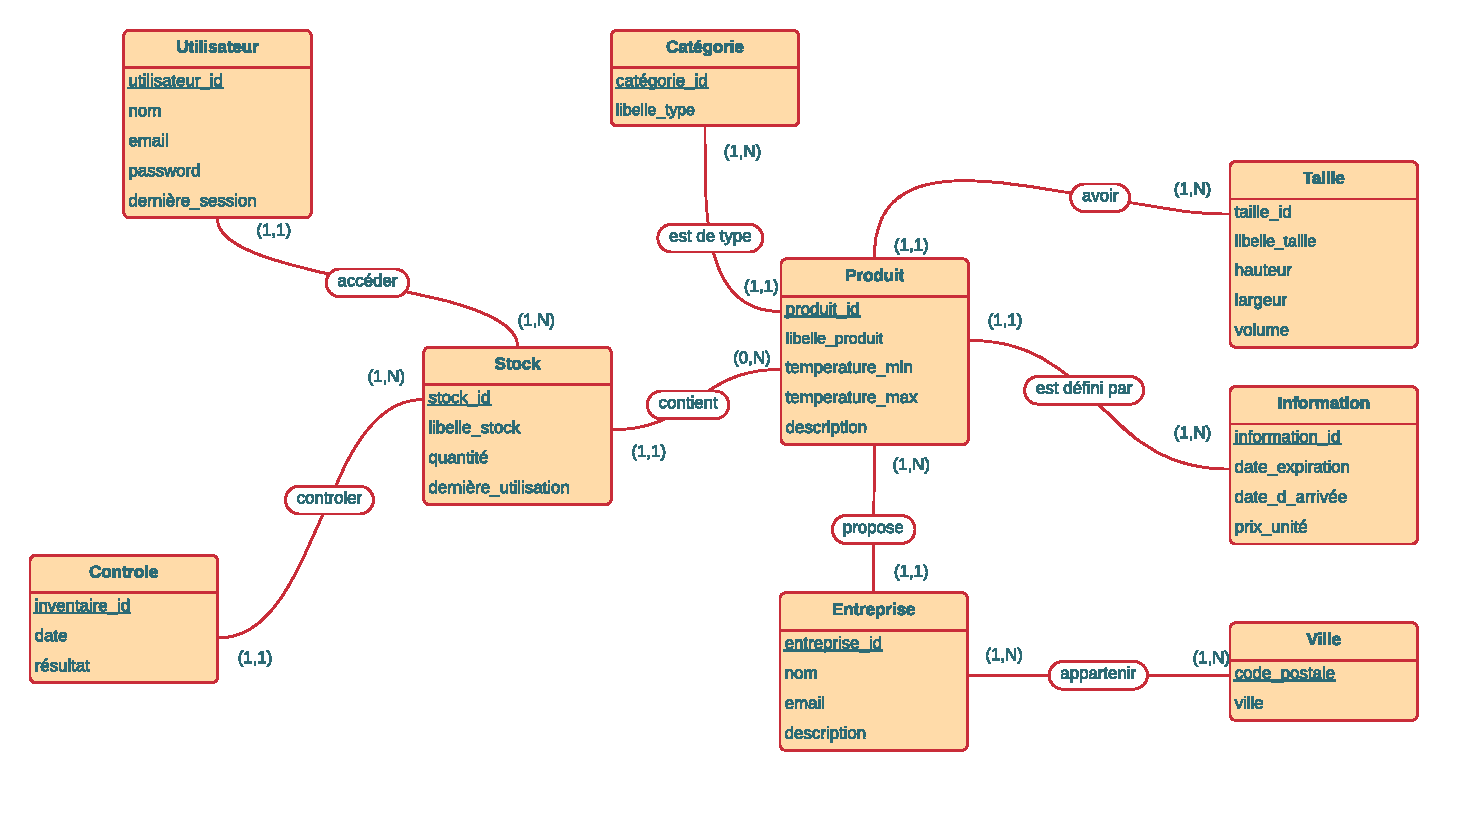
\includegraphics[keepaspectratio=true,scale=0.6]{Figures/mcd.pdf}
    \caption{Modèle EA}
    \label{fig:structure}
\end{figure}

\subsection{Description des entités}
Dans le diagramme entité-association, nous trouvons les entités suivantes :

\paragraph{Ville} Nous savons que chaque ville a son propre et unique code postal. C'est pourquoi nous pouvons le considérer ici comme étant une clé primaire.

\paragraph{Catégorie}
Une catégorie est définie par son identifiant, et son libellé. Nous avons choisi de le considérer comme une entité, au lieu de le mettre comme un attribut dans la table des produits. En effet, il existe de nombreux produits appartenant à la même catégorie (fruits, légumes, viande, etc.…).

\paragraph{Entreprise} Une entreprise est définie par son identifiant, son nom, email, et une brève description.

\paragraph{Utilisateur} Un utilisateur est défini par un identifiant, un nom d'utilisateur et un mot de passe pour accéder à son compte. De plus, pour garder une trace de ses activités, nous avons ajouté la date de la dernière session comme attribut.

\paragraph{Contrôle} Un contrôle est définit par un identifiant, un nom, la date de contrôle, ainsi que le résultat de contrôle.

\paragraph{Stock} Un stock est associé a un et un seul utilisateur. Il est définit par un identifiant unique, et un libellé.

\paragraph{Information} Il contient un certain nombre d'informations génériques et communes à de nombreux objets, comme la température du produit, la date d'expiration, le prix, la quantité, et la date d'entrée.

\paragraph{Taille} Elle fonctionne de la même manière que l'entité : "Information". L'entité "Taille"
contient des informations relatives à la forme géométrique de l'objet (hauteur, poids, volume).

\paragraph{Produit} Chaque produit est acheté auprès une où plusieurs entreprise. Il est définit par un identifiant unique, un libellé, une description, des informations uniques relative au produit comme la température du produit (la plus basse et la plus haute).


\section{Modèle logique de données (MLD)}
\subsection{Modèle relationnel}
Grâce au modèle conceptuel précédent, on a établi le modèle relationnel qui suit :

\paragraph{UTILISATEUR} (\textbf{\underline{utilisateur\_id}}, utilisateur\_nom, utilisateur\_email, utilisateur\_password, utilisateur\_dernière\_session, \#stock\_id)
\paragraph{STOCK} (\textbf{\underline{stock\_id}}, libellé\_stock, \#produit\_id)
\paragraph{CONTRÔLE} (\textbf{\underline{contrôle\_id}}, contrôle\_date, \#stock\_id)
\paragraph{PRODUIT} (\textbf{\underline{produit\_id}}, libellé\_produit, température\_max, température\_min, produit\_description, \#catégorie\_id, \#information\_id, \#taille\_id)
\paragraph{CATÉGORIE } (\textbf{\underline{catégorie\_id}}, libellé\_catégorie)
\paragraph{ENTREPRISE} (\textbf{\underline{entreprise\_id}}, entreprise\_nom, entreprise\_email, entreprise\_description, \#produit\_id)
\paragraph{VILLE} (\textbf{\underline{code\_postale}}, ville)
\paragraph{APPARTENIR} (\textbf{\underline{\#code\_postale, \#entreprise\_id}})
\paragraph{TAILLE} (\textbf{\underline{taille\_id}}, libellé\_taille, taille\_hauteur, taille\_largeur, taille\_volume)
\paragraph{INFORMATION} (\textbf{\underline{information\_id}}, date\_expiration, date\_d\_arrivée, prix\_unité, quantité)

\subsection{Dépendance fonctionnelle}

\begin{table}[H]
\resizebox{1.14\columnwidth}{!}{%
\begin{tabular}{lll}
\textbf{utilisateur\_id}&  $\longrightarrow$ &  \#stock\_id, utilisateur\_nom, utilisateur\_email, utilisateur\_password, \\
&& utilisateur\_dernière\_session \\
&&\\
\textbf{stock\_id}& $\longrightarrow$ & \#produit\_id, libellé\_stock \\
&&\\
\textbf{contrôle\_id}& $\longrightarrow$ & \#stock\_id, contrôle\_date \\
&&\\
\textbf{produit\_id}& $\longrightarrow$ & \#catégorie\_id, \#information\_id, \#taille\_id, libellé\_produit,\\
&& température\_max, température\_min, produit\_description \\
&&\\
\textbf{catégorie\_id}& $\longrightarrow$ & libellé\_catégorie \\
&&\\
\textbf{entreprise\_id}& $\longrightarrow$ & \#produit\_id, entreprise\_nom, entreprise\_email, entreprise\_description \\
&&\\
\textbf{code\_postale}& $\longrightarrow$ & ville \\
&&\\
(\textbf{\#code\_postale, \#entreprise\_id})& $\longrightarrow$ & \textit{évident.} \\
&&\\
\textbf{taille\_id}& $\longrightarrow$ & libellé\_taille, taille\_hauteur, taille\_largeur, taille\_volume \\
&&\\
\textbf{information\_id}& $\longrightarrow$ & date\_expiration, date\_d\_arrivée, prix\_unité, quantité
\end{tabular}
}
\end{table}


\subsection{Normalisation de la base en 3 forme normale}

\paragraph{UTILISATEUR} (\textbf{\underline{utilisateur\_id}}, utilisateur\_nom, utilisateur\_email, utilisateur\_password, utilisateur\_dernière\_session, \#stock\_id)

\texttt{utilisateur\_id} est le clé. En effet, toutes combinaison des attributs : \texttt{utilisateur\_nom, utilisateur\_email} et \texttt{utilisateur\_password} ne permet pas de retrouver les valeurs des autres attributs.

On a la $1^{\text{er}}$ forme normale (FN1). Car, tous les attributs sont atomiques. De plus, on a dépendance totale de la clé principale \texttt{utilisateur\_id}, ainsi, elle est aussi atomique. Donc, on a la $2^{\text{ème}}$ forme normale (FN2). Enfin, aucune combinaison entre les attributs ne suffissent pour déduire les autres attributs. On la $3^{\text{ème}}$ forme normale (FN3).

$\Longrightarrow\:$ \textbf{\textit{FN3 est respectée.}}

\paragraph{STOCK} (\textbf{\underline{stock\_id}}, libellé\_stock, \#produit\_id)

\texttt{stock\_id} est le clé. Car, tous les autres attributs dépendent fonctionnellement du clé \texttt{stock\_id}. Tous les attributs sont atomiques, on a bien la $1^{\text{er}}$ forme normale (FN1).

La clé est simple et non composite, et tous les autres attributs dépendent de la clé. Donc, on a la $2^{\text{ème}}$ forme normale (FN2). Ainsi, aucune combinaison entre les attributs ne suffissent pour déduire les autres attributs. On la $3^{\text{ème}}$ forme normale (FN3).

$\Longrightarrow\:$ \textbf{\textit{FN3 est respectée.}}

\paragraph{CONTRÔLE} (\textbf{\underline{contrôle\_id}}, contrôle\_date, \#stock\_id)

$\Longrightarrow\:$ \textbf{\textit{FN3 est respectée.}}

\paragraph{PRODUIT} (\textbf{\underline{produit\_id}}, libellé\_produit, température\_max, température\_min, produit\_description, \#catégorie\_id, \#information\_id, \#taille\_id)

\texttt{produit\_id} est le clé. Car, tous les autres attributs dépendent fonctionnellement du clé \texttt{produit\_id}. Tous les attributs sont atomiques, on a bien la $1^{\text{er}}$ forme normale (FN1).

La clé est simple et non composite, et tous les autres attributs dépendent de la clé. Donc, on a la $2^{\text{ème}}$ forme normale (FN2). Ainsi, aucune combinaison entre les attributs ne suffissent pour déduire les autres attributs. On la $3^{\text{ème}}$ forme normale (FN3).

$\Longrightarrow\:$ \textbf{\textit{FN3 est respectée.}}

\paragraph{CATÉGORIE } (\textbf{\underline{catégorie\_id}}, libellé\_catégorie)

$\Longrightarrow\:$ \textbf{\textit{FN3 est respectée.}}

\paragraph{ENTREPRISE} (\textbf{\underline{entreprise\_id}}, entreprise\_nom, entreprise\_email, entreprise\_description, \#produit\_id)

\texttt{entreprise\_id} est le clé. Car, tous les autres attributs dépendent fonctionnellement du clé \texttt{entreprise\_id}. Tous les attributs sont atomiques, on a bien la $1^{\text{er}}$ forme normale (FN1). De plus, on a dépendance totale de la clé principale. En effet, le clé est simple (non composite) et tous les autres attributs dépendent de la clé. On a donc le $2^{\text{ème}}$ forme normale (FN2). Enfin, on a $3^{\text{ème}}$ forme normale (FN3). Car, aucune combinaison entre les attributs ne suffissent pour déduire les autres attributs.

$\Longrightarrow\:$ \textbf{\textit{FN3 est respectée.}}



\paragraph{VILLE} (\textbf{\underline{code\_postale}}, ville)

On a la $1^{\text{er}}$ forme normale (FN1). En effet, tous les attributs sont atomiques, et l'identifiant \texttt{code\_postale} est unique. De plus, on a dépendance totale de la clé principale. En effet, le clé est simple (non composite) et l'attribut \texttt{ville} dépend de la clé. On a donc le $2^{\text{ème}}$ forme normale (FN2). On a $3^{\text{ème}}$ forme normale (FN3). Car, l'attribut \texttt{ville} dépend de la clé.

$\Longrightarrow\:$ \textbf{\textit{FN3 est respectée.}}

\paragraph{APPARTENIR} (\textbf{\underline{\#code\_postale, \#entreprise\_id}})

Les deux clés sont atomiques.

$\Longrightarrow\:$ \textbf{\textit{FN3 est respectée.}}é

\paragraph{TAILLE} (\textbf{\underline{taille\_id}}, libellé\_taille, taille\_hauteur, taille\_largeur, taille\_volume)

$\Longrightarrow\:$ \textbf{\textit{FN3 est respectée.}}

\paragraph{INFORMATION} (\textbf{\underline{information\_id}}, date\_expiration, date\_d\_arrivée, prix\_unité, quantité)

$\Longrightarrow\:$ \textbf{\textit{FN3 est respectée.}}
